\documentclass[a4paper,11pt]{article}

% Kodovani (cestiny) v dokumentu: utf-8
%\usepackage[cp1250]{inputenc}	% Omezena stredoevropska kodova stranka, pouze MSW.
\usepackage[utf8]{inputenc}	% Doporucujeme pouzivat UTF-8 (unicode).

\usepackage[margin=2cm]{geometry}
\newtoks\jmenopraktika \newtoks\jmeno \newtoks\datum
\newtoks\obor \newtoks\skupina \newtoks\rocnik \newtoks\semestr
\newtoks\cisloulohy \newtoks\jmenoulohy
\newtoks\tlak \newtoks\teplota \newtoks\vlhkost

\jmenopraktika={Fyzikální praktikum 1}
\jmeno={Lukáš Lejdar}
\datum={30. dubna 2023}
\obor={F}
\skupina={Út 16:00}

\cisloulohy={5}
\jmenoulohy={Měření modulu pružnosti pevných látek}

\tlak={101{,}35}
\teplota={21,1}
\vlhkost={47,7}


%%%%%%%%%%% Uzitecne balicky:
\usepackage[czech]{babel}

\usepackage{graphicx}
\usepackage{amsmath}
\usepackage{xspace}
\usepackage{url}
\usepackage{indentfirst}
\usepackage{wrapfig}
\usepackage{subcaption}
\usepackage{caption}
\usepackage{listings}
\usepackage{xcolor}


%%%%%% Zamezeni parchantu:
\widowpenalty 10000 \clubpenalty 10000 \displaywidowpenalty 10000
%%%%%% Parametry pro moznost vsazeni vetsiho poctu obrazku na stranku
\setcounter{topnumber}{3}	  % max. pocet floatu nahore (specifikace t)
\setcounter{bottomnumber}{3}	  % max. pocet floatu dole (specifikace b)
\setcounter{totalnumber}{6}	  % max. pocet floatu na strance celkem
\renewcommand\topfraction{0.9}	  % max podil stranky pro floaty nahore
\renewcommand\bottomfraction{0.9} % max podil stranky pro floaty dole
\renewcommand\textfraction{0.1}	  % min podil stranky, ktery musi obsahovat text
\intextsep=8mm \textfloatsep=8mm  %\intextsep pro ulozeni [h] floatu a \textfloatsep pro [b] or [t]

% Tecky za cisly sekci:
\renewcommand{\thesection}{\arabic{section}.}
\renewcommand{\thesubsection}{\thesection\arabic{subsection}.}
% Jednopismenna mezera mezi cislem a nazvem kapitoly:
\makeatletter \def\@seccntformat#1{\csname the#1\endcsname\hspace{1ex}} \makeatother
%
\newcommand{\vsn}[4]{\ensuremath{#1 =} #2(#3)\,#4}
\newcommand{\vrn}[6]{\ensuremath{#1 =} (#2 $\pm$ #3)\,#4 ($p=$ #5\,\%, $\nu=$ #6)}


%%%%%%%%%%%%%%%%%%%%%%%%%%%%%%%%%%%%%%%%%%%%%%%%%%%%%%%%%%%%%%%%%%%%%%%%%%%%%%%
% Zacatek dokumentu
%%%%%%%%%%%%%%%%%%%%%%%%%%%%%%%%%%%%%%%%%%%%%%%%%%%%%%%%%%%%%%%%%%%%%%%%%%%%%%%

\begin{document}

\thispagestyle{empty}

{
\begin{center}
\sf 
{\Large Ústav fyziky a technologií plazmatu Přírodovědecké fakulty Masarykovy univerzity} \\
\bigskip
{\huge \bfseries FYZIKÁLNÍ PRAKTIKUM} \\
\bigskip
{\Large \the\jmenopraktika}
\end{center}

\bigskip

\sf
\noindent
\setlength{\arrayrulewidth}{1pt}
\begin{tabular*}{\textwidth}{@{\extracolsep{\fill}} l l}
\large {\bfseries Zpracoval:}  \the\jmeno & \large  {\bfseries Naměřeno:} \the\datum\\[2mm]
\large  {\bfseries Obor:} \the\obor  \hspace{40mm}  {\bfseries Skupina:} \the\skupina %
&\large {\bfseries Testováno:}\\
\\
\hline
\end{tabular*}
}

\bigskip
{
\sf
\noindent \begin{tabular}{p{4cm} p{0.6\textwidth}}
\Large  Úloha č. {\bfseries \the\cisloulohy:} \par
\smallskip
$T=\the\teplota$~$^\circ$C \par
$p=\the\tlak$~kPa \par
$\varphi=\the\vlhkost$~\%
&\Large \bfseries \the\jmenoulohy  \\[2mm]
\end{tabular}
}

\vskip1cm

\section{Úvod}
 
V úloze budu měřit různé moduly pružnosti. Zavádíme je následujícím způsobem: \\

\noindent
Pro materiál v tahu platí v nejjednodušším případě Hookův zákon

\begin{equation}
\sigma_{\text{n}} = \frac{dF_{\text{n}}}{dS} = \frac{\Delta l}{l} E,
\end{equation}

\noindent
kde $\Delta$ l délkové prodloužení, l délka vzorku, $dF_{\text{n}}$ průmět síly na kolmici ke zvolené plošce dS, $\sigma_{n}$ normálové napětí a E modul pružnosti. Pokud je materiál v torzi místo v tahu a speciálně se zabýváme drátem o rozměrech l $\times$ $\rho$ $\times$ $2\pi$, bude platit velmi obdobný zákon

\begin{equation}
  \sigma_{\text{t}} = \frac{dF_{\text{t}}}{dS} = \frac{\rho \varphi}{a} G
\end{equation}

\noindent
kde $\varphi$ je úhel zkroucení konce drátu a G modul pružnosti ve smyku. 

\section{Postup měření}

\subsection{Měření modulu pružnosti v tahu přímou metodou z prodloužení \\ drátu}

\begin{wrapfigure}{r}{70pt}
  \vspace{-9.5em}
  \centering
  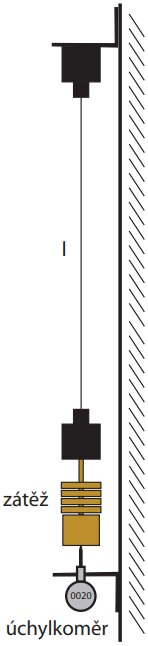
\includegraphics[width=53pt]{uchylkomer.jpg}
  \caption{Přímá metoda}
\end{wrapfigure}

  \vspace{1em}
% this text now overlaps with the title
Měření bude probíhat jako na obrázku 1. Z úchytu visí kolmo dolů drát o délce l a průměru d, který můžu postupně zatěžovat a úchylkoměrem  velmi citlivě měřit jeho prodloužení. \\

  Do Hookova zákona dosadím za S obsah průřezu drátu a za F gravitační sílu, kterou na drát působí závaží.

\begin{equation}
 \frac{4 g m}{\pi d^2} = \frac{\Delta l}{l} E
\end{equation}

Změřím odchylku pro každé další přidané závaží a modul pružnosti určím ze sklonu lineárního fitu hodnot.

\begin{equation}
  k = \frac{\Delta l}{m} = \frac{4 g l}{\pi d^2 E}
\end{equation}

\subsection{Měření modulu pružnosti v tahu z průhybu plného obdélníkového nosníku}

Měření bude probíhat jako na obrázku 2. Mezi dvěma podpěrami ve vzdálenosti l je položený obdélníkový nosník o rozměrech a $\times$ b $\times$ c, který můžu postupně zatěžovat přidáváním závaží a úchylkoměrem měřit výchylku y od původní polohy.

\begin{figure}[htpb]
  \centering
  \begin{subfigure}[b]{0.65\textwidth}
    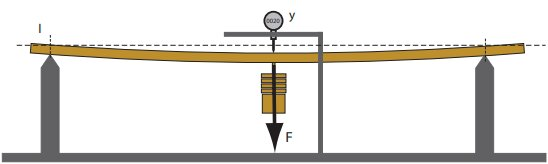
\includegraphics[width=\textwidth]{nosnik_pred.jpg}
  \end{subfigure}
  \begin{subfigure}[b]{70pt}
    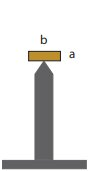
\includegraphics[width=51pt]{nosnik_bok.jpg}
  \end{subfigure}
  \caption{průhyb nosníku}
\end{figure}

Vztah mezi průhybem y daného nosníku a zatížením F=mg je

\begin{equation}
y = \frac{m g l^{3}}{4 E a^{3} b}
\end{equation}

Stejně jako v předešlém případě budu postupovat zvyšováním zátěže pro závislost y(m), kterou vyhodnotím fitem.

\subsection{Měření modulu pružnosti ve smyku dynamickou metodou}

Na homogenní drát délky l o poloměru r je zavěšena homogenní koule o poloměru R a hmotnosti m mnohem větší, než je hmotnost drátu. Když kouli pootočím kolem svislé osy, vykonává torzní kmity. Pokud zkroucení drátu odpovídá pružné torzní deformaci, pak platí vztah pro modul pružnosti ve~smyku G

\begin{equation}
  G = \frac{16 \pi m R^2 l}{5 r^{4} T^{2}}.
\end{equation}
\\
Přitom T je perioda kmitání. Provedu 10 měření doby 10 period kmitání, veličiny zprůměruju a dopočítám G.

\begin{figure}[htpb]
  \centering
  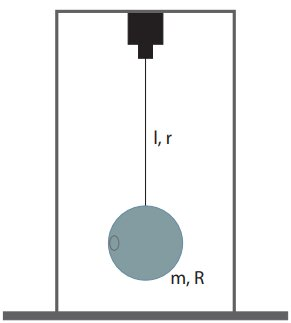
\includegraphics[width=0.38\textwidth]{oscilator.jpg}
  \caption{Torzní oscilátor}
\end{figure}

\section{Výsledky měření}

\subsection{Měření modulu pružnosti v tahu přímou metodou z prodloužení drátu}

Na svislý ocelový drát o průměru d a délce l = 1567 mm jsem postupně přidával závaží a měřil prodloužení $\Delta l$. Získané hodnoty jsou uvedené v grafu 4. Dosazením do vztahu (4) dostávám modul pružnosti drátu E. Pro výpočet nejistoty jsem použil python script uvedený v příloze 1.

\captionsetup[figure]{name=Graf,justification=centering,format=plain}
\captionsetup[table]{name=Tabulka,justification=centering,format=plain}

\begin{table}[htpb]
  \begin{minipage}{0.62\linewidth}
    \centering
    % GNUPLOT: LaTeX picture with Postscript
\begingroup
  \makeatletter
  \providecommand\color[2][]{%
    \GenericError{(gnuplot) \space\space\space\@spaces}{%
      Package color not loaded in conjunction with
      terminal option `colourtext'%
    }{See the gnuplot documentation for explanation.%
    }{Either use 'blacktext' in gnuplot or load the package
      color.sty in LaTeX.}%
    \renewcommand\color[2][]{}%
  }%
  \providecommand\includegraphics[2][]{%
    \GenericError{(gnuplot) \space\space\space\@spaces}{%
      Package graphicx or graphics not loaded%
    }{See the gnuplot documentation for explanation.%
    }{The gnuplot epslatex terminal needs graphicx.sty or graphics.sty.}%
    \renewcommand\includegraphics[2][]{}%
  }%
  \providecommand\rotatebox[2]{#2}%
  \@ifundefined{ifGPcolor}{%
    \newif\ifGPcolor
    \GPcolorfalse
  }{}%
  \@ifundefined{ifGPblacktext}{%
    \newif\ifGPblacktext
    \GPblacktexttrue
  }{}%
  % define a \g@addto@macro without @ in the name:
  \let\gplgaddtomacro\g@addto@macro
  % define empty templates for all commands taking text:
  \gdef\gplbacktext{}%
  \gdef\gplfronttext{}%
  \makeatother
  \ifGPblacktext
    % no textcolor at all
    \def\colorrgb#1{}%
    \def\colorgray#1{}%
  \else
    % gray or color?
    \ifGPcolor
      \def\colorrgb#1{\color[rgb]{#1}}%
      \def\colorgray#1{\color[gray]{#1}}%
      \expandafter\def\csname LTw\endcsname{\color{white}}%
      \expandafter\def\csname LTb\endcsname{\color{black}}%
      \expandafter\def\csname LTa\endcsname{\color{black}}%
      \expandafter\def\csname LT0\endcsname{\color[rgb]{1,0,0}}%
      \expandafter\def\csname LT1\endcsname{\color[rgb]{0,1,0}}%
      \expandafter\def\csname LT2\endcsname{\color[rgb]{0,0,1}}%
      \expandafter\def\csname LT3\endcsname{\color[rgb]{1,0,1}}%
      \expandafter\def\csname LT4\endcsname{\color[rgb]{0,1,1}}%
      \expandafter\def\csname LT5\endcsname{\color[rgb]{1,1,0}}%
      \expandafter\def\csname LT6\endcsname{\color[rgb]{0,0,0}}%
      \expandafter\def\csname LT7\endcsname{\color[rgb]{1,0.3,0}}%
      \expandafter\def\csname LT8\endcsname{\color[rgb]{0.5,0.5,0.5}}%
    \else
      % gray
      \def\colorrgb#1{\color{black}}%
      \def\colorgray#1{\color[gray]{#1}}%
      \expandafter\def\csname LTw\endcsname{\color{white}}%
      \expandafter\def\csname LTb\endcsname{\color{black}}%
      \expandafter\def\csname LTa\endcsname{\color{black}}%
      \expandafter\def\csname LT0\endcsname{\color{black}}%
      \expandafter\def\csname LT1\endcsname{\color{black}}%
      \expandafter\def\csname LT2\endcsname{\color{black}}%
      \expandafter\def\csname LT3\endcsname{\color{black}}%
      \expandafter\def\csname LT4\endcsname{\color{black}}%
      \expandafter\def\csname LT5\endcsname{\color{black}}%
      \expandafter\def\csname LT6\endcsname{\color{black}}%
      \expandafter\def\csname LT7\endcsname{\color{black}}%
      \expandafter\def\csname LT8\endcsname{\color{black}}%
    \fi
  \fi
    \setlength{\unitlength}{0.0500bp}%
    \ifx\gptboxheight\undefined%
      \newlength{\gptboxheight}%
      \newlength{\gptboxwidth}%
      \newsavebox{\gptboxtext}%
    \fi%
    \setlength{\fboxrule}{0.5pt}%
    \setlength{\fboxsep}{1pt}%
    \definecolor{tbcol}{rgb}{1,1,1}%
\begin{picture}(5472.00,3168.00)%
    \gplgaddtomacro\gplbacktext{%
      \csname LTb\endcsname%%
      \put(-78,158){\makebox(0,0)[r]{\strut{}$0$}}%
      \put(-78,699){\makebox(0,0)[r]{\strut{}$0.1$}}%
      \put(-78,1241){\makebox(0,0)[r]{\strut{}$0.2$}}%
      \put(-78,1782){\makebox(0,0)[r]{\strut{}$0.3$}}%
      \put(-78,2323){\makebox(0,0)[r]{\strut{}$0.4$}}%
      \put(-78,2864){\makebox(0,0)[r]{\strut{}$0.5$}}%
      \put(54,-62){\makebox(0,0){\strut{}$0$}}%
      \put(948,-62){\makebox(0,0){\strut{}$200$}}%
      \put(1841,-62){\makebox(0,0){\strut{}$400$}}%
      \put(2735,-62){\makebox(0,0){\strut{}$600$}}%
      \put(3629,-62){\makebox(0,0){\strut{}$800$}}%
      \put(4522,-62){\makebox(0,0){\strut{}$1000$}}%
      \put(5416,-62){\makebox(0,0){\strut{}$1200$}}%
      \put(277,2864){\makebox(0,0)[l]{\strut{}k = $(449 \pm 4) \cdot 10^{-6}$ mkg$^{-1}$}}%
    }%
    \gplgaddtomacro\gplfronttext{%
      \csname LTb\endcsname%%
      \put(4501,721){\makebox(0,0)[r]{\strut{}fit f(m) = k$\cdot$m}}%
      \csname LTb\endcsname%%
      \put(4501,521){\makebox(0,0)[r]{\strut{}přidávání závaží}}%
      \csname LTb\endcsname%%
      \put(4501,321){\makebox(0,0)[r]{\strut{}odébírání závaží}}%
      \csname LTb\endcsname%%
      \put(-683,1646){\rotatebox{-270.00}{\makebox(0,0){\strut{}$\Delta l$ (mm)}}}%
      \put(2735,-392){\makebox(0,0){\strut{}m (g)}}%
    }%
    \gplbacktext
    \put(0,0){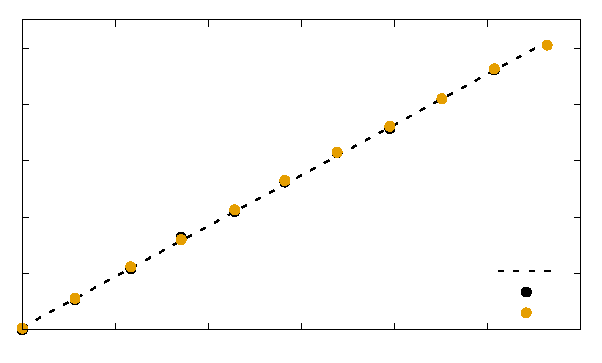
\includegraphics[width={273.60bp},height={158.40bp}]{prodlouzeni}}%
    \gplfronttext
  \end{picture}%
\endgroup

    \captionof{figure}{Závislost prodloužení drátu na hmotnosti závaží}
  \end{minipage}
  \hfill
  \begin{minipage}{0.30\linewidth}
    \centering
    \begin{tabular}{|c|c|}
      \hline
      n & d (mm) \\
      \hline
      1 & 0.50 \\
      2 & 0.50 \\
      3 & 0.50 \\
      4 & 0.50 \\
      5 & 0.51 \\
      6 & 0.50 \\
      7 & 0.49 \\
      8 & 0.50 \\
      9 & 0.49 \\
      10 & 0.50 \\
      \hline
      x & $(0.499 \pm 0.007)$ \\
      \hline
    \end{tabular}
    \caption{měření průměru drátu mikrometrem}
  \end{minipage}
\end{table}
\vspace{-10pt}
\begin{center}
 \vrn{E}{175}{5}{GPa}{99.73}{9} 
\end{center}

\subsection{Měření modulu pružnosti v tahu z průhybu plného obdélníkového nosníku}

Na obdélníkové nosníky o rozměrech a $\times$ b $\times$ c (tabulka 2) jsem postupně přidával závaží a měřil prohnutí~y. Získané hodnoty jsou uvedené v grafu 5, python script pro výpočet v příloze 2 a výsledné moduly pružnosti v tabulce 2. Vzdálenost břitů l = ($89.9\pm0.03$) cm jsem změřil pravítkem.

\begin{figure}[htpb]
  \centering
  % GNUPLOT: LaTeX picture with Postscript
\begingroup
  \makeatletter
  \providecommand\color[2][]{%
    \GenericError{(gnuplot) \space\space\space\@spaces}{%
      Package color not loaded in conjunction with
      terminal option `colourtext'%
    }{See the gnuplot documentation for explanation.%
    }{Either use 'blacktext' in gnuplot or load the package
      color.sty in LaTeX.}%
    \renewcommand\color[2][]{}%
  }%
  \providecommand\includegraphics[2][]{%
    \GenericError{(gnuplot) \space\space\space\@spaces}{%
      Package graphicx or graphics not loaded%
    }{See the gnuplot documentation for explanation.%
    }{The gnuplot epslatex terminal needs graphicx.sty or graphics.sty.}%
    \renewcommand\includegraphics[2][]{}%
  }%
  \providecommand\rotatebox[2]{#2}%
  \@ifundefined{ifGPcolor}{%
    \newif\ifGPcolor
    \GPcolorfalse
  }{}%
  \@ifundefined{ifGPblacktext}{%
    \newif\ifGPblacktext
    \GPblacktexttrue
  }{}%
  % define a \g@addto@macro without @ in the name:
  \let\gplgaddtomacro\g@addto@macro
  % define empty templates for all commands taking text:
  \gdef\gplbacktext{}%
  \gdef\gplfronttext{}%
  \makeatother
  \ifGPblacktext
    % no textcolor at all
    \def\colorrgb#1{}%
    \def\colorgray#1{}%
  \else
    % gray or color?
    \ifGPcolor
      \def\colorrgb#1{\color[rgb]{#1}}%
      \def\colorgray#1{\color[gray]{#1}}%
      \expandafter\def\csname LTw\endcsname{\color{white}}%
      \expandafter\def\csname LTb\endcsname{\color{black}}%
      \expandafter\def\csname LTa\endcsname{\color{black}}%
      \expandafter\def\csname LT0\endcsname{\color[rgb]{1,0,0}}%
      \expandafter\def\csname LT1\endcsname{\color[rgb]{0,1,0}}%
      \expandafter\def\csname LT2\endcsname{\color[rgb]{0,0,1}}%
      \expandafter\def\csname LT3\endcsname{\color[rgb]{1,0,1}}%
      \expandafter\def\csname LT4\endcsname{\color[rgb]{0,1,1}}%
      \expandafter\def\csname LT5\endcsname{\color[rgb]{1,1,0}}%
      \expandafter\def\csname LT6\endcsname{\color[rgb]{0,0,0}}%
      \expandafter\def\csname LT7\endcsname{\color[rgb]{1,0.3,0}}%
      \expandafter\def\csname LT8\endcsname{\color[rgb]{0.5,0.5,0.5}}%
    \else
      % gray
      \def\colorrgb#1{\color{black}}%
      \def\colorgray#1{\color[gray]{#1}}%
      \expandafter\def\csname LTw\endcsname{\color{white}}%
      \expandafter\def\csname LTb\endcsname{\color{black}}%
      \expandafter\def\csname LTa\endcsname{\color{black}}%
      \expandafter\def\csname LT0\endcsname{\color{black}}%
      \expandafter\def\csname LT1\endcsname{\color{black}}%
      \expandafter\def\csname LT2\endcsname{\color{black}}%
      \expandafter\def\csname LT3\endcsname{\color{black}}%
      \expandafter\def\csname LT4\endcsname{\color{black}}%
      \expandafter\def\csname LT5\endcsname{\color{black}}%
      \expandafter\def\csname LT6\endcsname{\color{black}}%
      \expandafter\def\csname LT7\endcsname{\color{black}}%
      \expandafter\def\csname LT8\endcsname{\color{black}}%
    \fi
  \fi
    \setlength{\unitlength}{0.0500bp}%
    \ifx\gptboxheight\undefined%
      \newlength{\gptboxheight}%
      \newlength{\gptboxwidth}%
      \newsavebox{\gptboxtext}%
    \fi%
    \setlength{\fboxrule}{0.5pt}%
    \setlength{\fboxsep}{1pt}%
    \definecolor{tbcol}{rgb}{1,1,1}%
\begin{picture}(8640.00,4320.00)%
    \gplgaddtomacro\gplbacktext{%
      \csname LTb\endcsname%%
      \put(-46,216){\makebox(0,0)[r]{\strut{}$0$}}%
      \put(-46,796){\makebox(0,0)[r]{\strut{}$1$}}%
      \put(-46,1376){\makebox(0,0)[r]{\strut{}$2$}}%
      \put(-46,1956){\makebox(0,0)[r]{\strut{}$3$}}%
      \put(-46,2535){\makebox(0,0)[r]{\strut{}$4$}}%
      \put(-46,3115){\makebox(0,0)[r]{\strut{}$5$}}%
      \put(-46,3695){\makebox(0,0)[r]{\strut{}$6$}}%
      \put(-46,4275){\makebox(0,0)[r]{\strut{}$7$}}%
      \put(86,-4){\makebox(0,0){\strut{}$0$}}%
      \put(1497,-4){\makebox(0,0){\strut{}$200$}}%
      \put(2908,-4){\makebox(0,0){\strut{}$400$}}%
      \put(4319,-4){\makebox(0,0){\strut{}$600$}}%
      \put(5730,-4){\makebox(0,0){\strut{}$800$}}%
      \put(7141,-4){\makebox(0,0){\strut{}$1000$}}%
      \put(8552,-4){\makebox(0,0){\strut{}$1200$}}%
    }%
    \gplgaddtomacro\gplfronttext{%
      \csname LTb\endcsname%%
      \put(1913,4001){\makebox(0,0)[r]{\strut{}přidávání závaží}}%
      \csname LTb\endcsname%%
      \put(1913,3801){\makebox(0,0)[r]{\strut{}odebírání závaží}}%
      \csname LTb\endcsname%%
      \put(1913,3601){\makebox(0,0)[r]{\strut{}hliník}}%
      \csname LTb\endcsname%%
      \put(1913,3401){\makebox(0,0)[r]{\strut{}mosaz}}%
      \csname LTb\endcsname%%
      \put(1913,3201){\makebox(0,0)[r]{\strut{}měď}}%
      \csname LTb\endcsname%%
      \put(1913,3001){\makebox(0,0)[r]{\strut{}ocel}}%
      \csname LTb\endcsname%%
      \put(-387,2245){\rotatebox{-270.00}{\makebox(0,0){\strut{}y (mm)}}}%
      \put(4319,-334){\makebox(0,0){\strut{}m (g)}}%
    }%
    \gplgaddtomacro\gplbacktext{%
    }%
    \gplgaddtomacro\gplfronttext{%
      \csname LTb\endcsname%%
      \put(1755,4001){\makebox(0,0)[r]{\strut{} }}%
    }%
    \gplgaddtomacro\gplbacktext{%
    }%
    \gplgaddtomacro\gplfronttext{%
      \csname LTb\endcsname%%
      \put(1860,4001){\makebox(0,0)[r]{\strut{} }}%
    }%
    \gplgaddtomacro\gplbacktext{%
    }%
    \gplgaddtomacro\gplfronttext{%
      \csname LTb\endcsname%%
      \put(1966,4001){\makebox(0,0)[r]{\strut{} }}%
    }%
    \gplgaddtomacro\gplbacktext{%
    }%
    \gplgaddtomacro\gplfronttext{%
      \csname LTb\endcsname%%
      \put(2072,4001){\makebox(0,0)[r]{\strut{} }}%
    }%
    \gplbacktext
    \put(0,0){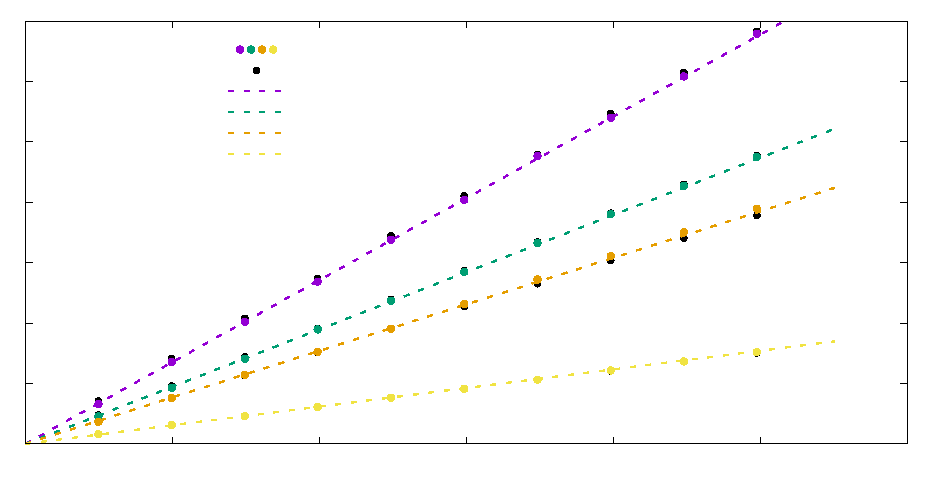
\includegraphics[width={432.00bp},height={216.00bp}]{nosnik}}%
    \gplfronttext
  \end{picture}%
\endgroup

  \caption{Závislost prohnutí nosníku na hmotnosti závaží.}
\end{figure}

\begin{table}[h]
  \centering
  \begin{tabular}{| c | c | c | c | c | c | c | c | c |}
    \hline
    materiál & \multicolumn{2}{| c |}{dural} & \multicolumn{2}{| c |}{mosaz} & \multicolumn{2}{| c |}{měď} & \multicolumn{2}{| c |}{ocel} \\ \hline
    rozměry & a (mm) & b (cm) & a (mm) & b (cm) & a (mm) & b (cm) & a (mm) & b (cm) \\ \hline
    1 & 5.04 & 3.030 & 5.06 & 3.008 & 5.04 & 3.022 & 5.75 & 2.980 \\ 
    2 & 5.04 & 3.028 & 5.05 & 3.012 & 5.06 & 3.010 & 5.75 & 2.978 \\ 
    3 & 5.04 & 3.022 & 5.06 & 3.022 & 5.10 & 3.032 & 5.77 & 2.980 \\ 
    4 & 5.03 & 3.020 & 5.06 & 3.014 & 5.04 & 3.024 & 5.76 & 2.988 \\ 
    5 & 5.03 & 3.040 & 5.06 & 3.016 & 5.03 & 3.010 & 5.75 & 2.982 \\ 
    6 & 5.04 & 3.022 & 5.06 & 3.012 & 5.04 & 3.080 & 5.75 & 2.986 \\ 
    7 & 5.02 & 3.020 & 5.06 & 3.080 & 5.02 & 3.120 & 5.76 & 2.980 \\ 
    8 & 5.03 & 3.036 & 5.06 & 3.010 & 5.04 & 3.120 & 5.75 & 2.982 \\ 
    9 & 5.04 & 3.020 & 5.06 & 3.008 & 5.04 & 3.160 & 5.75 & 2.984 \\ 
    10 & 5.02 & 3.016 & 5.06 & 3.012 & 5.05 & 3.020 & 5.75 & 2.982 \\ \hline
  \end{tabular}
  \caption{Měření rozměrů nosníků}
\end{table}
\begin{table}[h]
  \centering
  \begin{tabular}{| c | c | c | c | c |}
    \hline
    materiál & a (mm) & b (cm) & k ( $\mu$m kg$^{-1}$) & E (GPa) \\\hline
    dural & 5.03 $\pm$ 0.01 & 3.03 $\pm$ 0.01 & 6800 $\pm$ 8 & 67.9 $\pm$ 0.5 \\
    mosaz & 5.059 $\pm$ 0.004 & 3.02 $\pm$ 0.03 & 4770 $\pm$ 5 & 95.6 $\pm$ 0.9 \\
    měď & 5.05 $\pm$ 0.03 & 3.06 $\pm$ 0.07 & 3894 $\pm$ 9 & 116 $\pm$ 3 \\
    ocel & 5.754 $\pm$ 0.009 & 2.982 $\pm$ 0.004 & 1528 $\pm$ 2 & 205 $\pm$ 1 \\\hline
  \end{tabular}
  \caption{Vypočítané moduly pružnosti E z rozměrů nosníků. ($p=$ 99.73\,\%, $\nu=$ 9)  }
\end{table}

\subsection{Měření modulu pružnosti ve smyku dynamickou metodou}

Železná koule o poloměru D a hmotnosti m = 5.905 kg je zavěšená na drátě o průměru d a délce  l~=~51.450 $\pm$ 0.003 cm. Vychýlil jsem kouli a pokaždé změřil dobu deseti period T. Pro výpočet modulu pružnosti ze vztahu (6) jsem použil python script z přílohy 3.

\begin{table}[h]
 \centering
 \begin{tabular}{| c | c | c | c |}
    \hline
    měření & d (mm) & D (mm) & 10 $\cdot$ T (s) \\ 
    \hline
    1 & 1.00 & 99.60 & 39.89 \\
    2 & 0.99 & 99.70 & 39.81 \\
    3 & 0.99 & 99.80 & 39.56 \\
    4 & 0.99 & 99.78 & 40.05 \\
    5 & 0.99 & 99.70 & 39.64 \\
    6 & 0.99 & 99.80 & 39.94 \\
    7 & 1.00 & 99.72 & 39.82 \\
    8 & 0.99 & 99.78 & 39.94 \\
    9 & 0.99 & 99.76 & 39.93 \\
    10 & 1.00 & 99.76 & 39.72 \\
    \hline
    x & 0.993 $\pm$ 0.006 & 99.74 $\pm$ 0.08 & 39.8 $\pm$ 0.2 \\
    \hline
 \end{tabular}
 \caption{ Měření poloměru drátu a na něm zavěšené koule. ($p=$ 99.73\,\%, $\nu=$ 9)}
\end{table}

\begin{center}
  \vrn{G}{79}{2}{GPa}{99.73}{9}
\end{center}

\section{Závěr}

Z prodloužení ocelového drátu jsem změřil modul pružnosti E = $(175 \pm 5)$ GPa. Ne celkové nejistotě se podílela nejistota měření průměru drátu mikrometrem a nejistota sklonu lineárního fitu hodnot.  \\

Metodou prohnutí nosníků jsem změřil moduly pružnosti hliníku, mědi, mosazi a ocele a výsledné hodnoty uvedl v tabulce 3. Pro všechny čtyři kovy je rozdíl oproti tabulkám z odkazu [1] v řádech několika procent. Metoda průhybu nosníku dosáhla mnohem přesnějšího výsledku, než přímá metoda měření z prodloužení drátu. \\

Pomocí periody torzních kmitů jsem změřil modul pružnosti ve smyku ocelového drátu \linebreak \mbox{G = $(79\pm2)$ GPa.} Nepřesnost měření je převážně způsobená nejistotou periody kmitání. Bylo by potřeba místo manuálního spouštění stopek použít nějakou přesnější metodu. Tabulková hodnota je 79.3 GPa. \\

\begin{thebibliography}{0}
\bibitem{moduly_pruznosti} Tabulky Youngových modulů pružnosti ~\url{http://kabinet.fyzika.net/studium/tabulky/modul-pruznosti.php}.   
\bibitem{navod_k_uloze} návod k úloze \url{https://www.physics.muni.cz/kof/vyuka/fp1_05.pdf}
\end{thebibliography}

\definecolor{backcolour}{rgb}{0.95,0.95,0.92}

\lstset{
    backgroundcolor=\color{backcolour},   
    basicstyle=\ttfamily\footnotesize,
    breakatwhitespace=false,         
    breaklines=true,                 
    captionpos=b,                    
    keepspaces=true,                 
    numbers=left,                    
    numbersep=5pt,                  
    showspaces=false,                
    showstringspaces=false,
    showtabs=false,                  
    tabsize=2
}

\section{Přílohy}

\begin{lstlisting}[caption={Výpočet modulu pružnosti v tahu přímou metodou }]
import numpy as np
import uncertainties as unc
import math

d = np.array([ 0.50, 0.50, 0.50, 0.50, 0.51, 0.50, 0.49, 0.50, 0.49, 0.50 ]) * 0.001
d = unc.ufloat(np.mean(d), np.std(d) * 4.094)
k = unc.ufloat(449, 4) * 1e-6
l = 1567 * 0.001

print(4 * 9.81 * l / (math.pi * d ** 2 * k))
\end{lstlisting}

\begin{lstlisting}[caption={Výpočet modulů pružností nosníků}]
import uncertainties as unc
import numpy as np
import scipy.stats as stats
import math

def kf(ddof):
  return stats.t.ppf(0.5 + 0.9973 / 2, df=ddof)

def E(b, a, k):
  k = unc.ufloat(k[0], k[1]) * 1e-6 
  a = unc.ufloat(np.mean(a), np.std(a,ddof=1)/math.sqrt(len(a))*kf(len(a)-1))*1e-3
  b = unc.ufloat(np.mean(b), np.std(b,ddof=1)/math.sqrt(len(b))*kf(len(b)-1))*1e-2
  l = unc.ufloat(89.9, 0.03) * 0.01

  return 9.809980 * l**3 / (4 * k * a ** 3 * b)

table = np.loadtxt("nosniky_rozmery.txt")
print('dural', E(table[:, 0], table[:, 1], (6800, 8)))
print('mosaz', E(table[:, 4], table[:, 5], (4770, 5)))
print('med' E(table[:, 2], table[:, 3], (3894, 9)))
print('ocel', E(table[:, 6], table[:, 7], (1528, 2)))
\end{lstlisting}

\begin{lstlisting}[caption={Výpočet modulu pružnosti dynamickou metodou}]
import uncertainties as unc
import math
import numpy as np
import scipy.stats as stats

def k(ddof):
    return stats.t.ppf(0.5 + 0.9973 / 2, df=ddof)

table = np.loadtxt("oscilator_rozmery.txt")
d = table[:, 0]
D = table[:, 1]
T = table[:, 2]

d = unc.ufloat(np.mean(d), np.std(d, ddof=1) / math.sqrt(len(d)) * k(len(d)-1))*1e-3
D = unc.ufloat(np.mean(D), np.std(D, ddof=1) / math.sqrt(len(D)) * k(len(D)-1))*1e-3
T = unc.ufloat(np.mean(T), np.std(T, ddof=1) / math.sqrt(len(T)) * k(len(T)-1))/10.0
l = unc.ufloat(51.45, 0.003) * 0.01
m = 5.905

print(16 * math.pi * m * (D/2) ** 2 * l / (5 * (d/2) ** 4 * T ** 2))
  
\end{lstlisting}

\end{document}

\end{document}
